\documentclass{ctexart}


\author{李约瀚 \\ 14130140331 \\ qinka@live.com \\ qinka@qinka.pw}
\title{FPGA设计基础实验报告 (一)}

\usepackage{listings}

%\lstset{frame=single,breaklines,numbers}

\begin{document}
    
        % Cover
        \thispagestyle{empty}
        \begin{center}
            \vspace*{4em}
            {\Huge\textbf{FPGA设计基础实验报告\\\vspace*{0.5em} (一)}}
            \vfill
            \begin{tabular}{c@{:}l}
                班级 & 1413014 \\
                学号 & 14130140331 \\ 
                姓名 & 李约瀚 \\ 
                教师 & 沈沛意 \\
            \end{tabular} 
            \vspace*{4em}\\
        \end{center}
        \newpage
        
       
        % Setting
        \setcounter{page}{0}
        \setcounter{section}{0}
        %\renewcommand\thesection{实验编号 1-\numeric{section} 题目: }
        %\renewcommand\thesubsection{}
        %\renewcommand\thesubsubsection{(\numeric{subsubsection})}

        %% Exp 1-1
        \section{控制二极管循环发光}
        
        \subsection{实验目的}
        \begin{enumerate}
        \item 熟悉 ISE 软件,会使用ISE软件进行设计和仿真
        \item 学会程序下载
        \end{enumerate}

        \subsection{实验内容}

        \begin{enumerate}
        \item 创建工程
        \item 设计输入
        \item 综合实现
        \item 进行硬件配置
        \end{enumerate}

        \subsection{报告正文}

        \subsubsection{实验原理}
        
        根据 Nexys3 的指引手册,Nexys3 开发板上有8个并排放置的发光二极管,从左到右分别标注的是LD0~LD7,
        实验要求其中一个二极管发光,其他7个二极管均处于截止状态。二极管发光的顺序按照向左或者向右的方向,并有波动开关SW0控制方向。
        
        \subsubsection{实验过程}

        \paragraph{新建工程}

        打开 ISE 14.7之后,选择新建工程,将工程的路径设置好。
        在单击下一步之后,选择 Nexys3 的 Spartan6 XC6SLX16-CS324 芯片对应的配置。硬件描述语言选择 Verilog,其中的设计硬件用的描述语言是 Verilog。
        然后点击下一步之后进入工程信息页面并确认无误之后,点击完成结束工程的创建。

        \paragraph{设计输入}

        在菜单 \verb|Project| 中选择 \verb|New Source| 创建新的设计,并选择 \verb|Verilog Module| 创建文件。
        
        其中输入的设计文件是
\begin{lstlisting}[language=Verilog]
`timescale 1ns / 1ps
// Copyright (C) Xilinx
module led_shift(
    input clk,
    input reset,
    input dir_r_l,
    output [7:0] led
    );
	 
	reg [7:0] led;
	reg [28:0] cnt;	//计数分频器
	always @ (posedge clk or posedge reset) begin
		if(reset) begin
			cnt <= 29'd0;
		end
		else begin
			if(cnt == 29'd99_999_999) begin
				cnt <= 29'd0;
			end
			else begin
				cnt <= cnt + 1;
			end
		end
	end
	
	reg new_second;	//得到一秒的信号
	always @ (posedge clk or posedge reset) begin
		if(reset) begin
			new_second <= 1'b0;
		end
		else begin
			if(cnt == 29'd99_999_999) begin
				new_second <= 1'b1;
			end
			else if(new_second) begin
				new_second <= 1'b0;
			end
		end
	end
	
	//控制二极管循环发光
	always @ (posedge clk or posedge reset) begin
		if(reset) begin	
			led <= 8'b0000_0001;
		end
		else begin
			if(new_second) begin
				if(dir_r_l == 1'b1) begin	//向右移动
					led <= {led[0], led[7:1]};
				end
				else begin	//向左移动
					led <= {led[6:0], led[7]};
				end
			end
		end
	end

endmodule
\end{lstlisting}

        \paragraph{综合与实现}

		在左侧的 \verb|Design| 面板中下方中 双击 \verb|Synthesize-XST| 开始综合过程。
		

        在左侧的 \verb|Design| 面板中的 \verb|Hierarchy| 中选中创建的 HDL 源文件,在下方的双击 \verb|View RTL Schematic| 查看电路。

        \begin{figure}
\centering
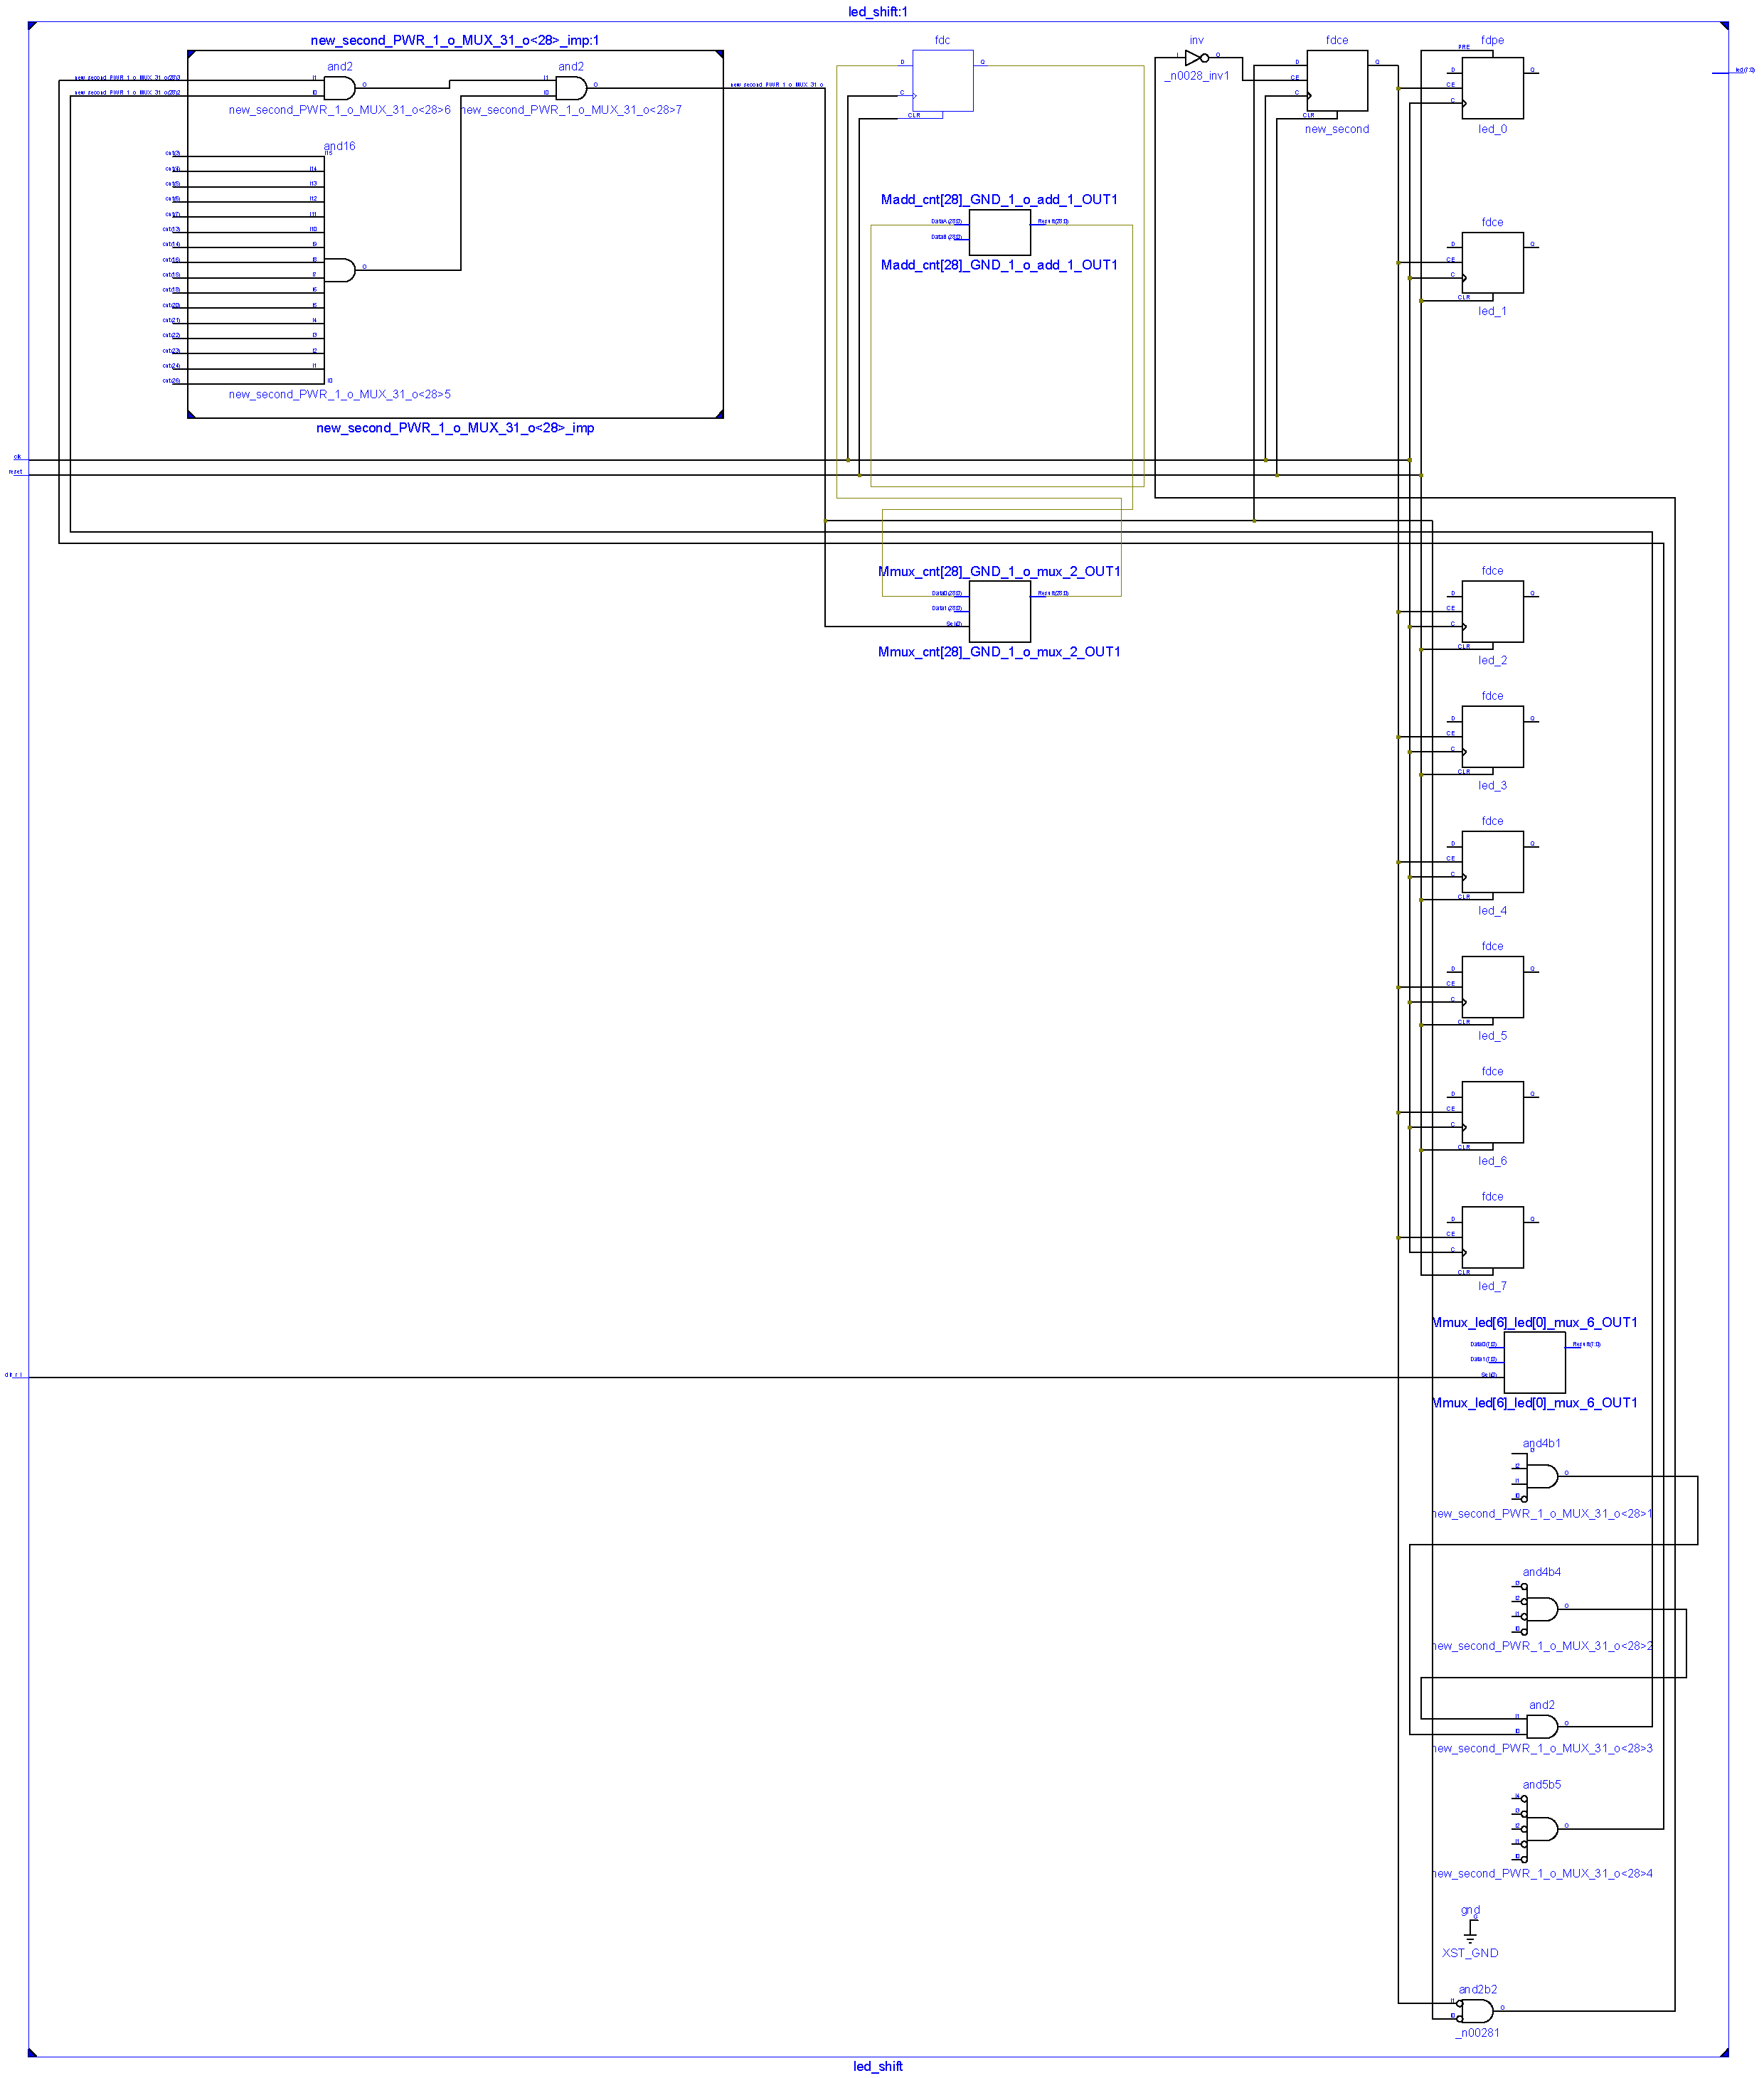
\includegraphics[width=0.7\linewidth]{report1-circiut-1.eps}
\caption[Circuit]{}
\label{fig:report1-circiut-1}
\end{figure}

        之后添加用户约束文件,这个文件使得器件脚针与外围设备可以绑定,链接。
        添加的方式可以在 \verb|Design| 面板中找到 带有 \verb|Pre| 前缀的 \verb|PlanAhead| 中配置脚针。或者为工程添加用户约束文件。
		
        用户约束文件的内容大致是配置脚针(site) 与外围设备的链接配置。
\begin{lstlisting}
Net "clk"      LOC = V10;
Net "reset"  LOC = C9;
Net "dir_r_l" LOC = T10;
Net "clk"      IOSTANDARD = LVCMOS33;
Net  "reset" IOSTANDARD = LVCMOS33;
Net "dir_r_l" IOSTANDARD = LVCMOS33;

Net "led[0]" LOC = U16;
Net "led[1]" LOC = V16;
Net "led[2]" LOC = U15;
Net "led[3]" LOC = V15;
Net "led[4]" LOC = M11;
Net "led[5]" LOC = N11;
Net "led[6]" LOC = R11;
Net "led[7]" LOC = T11;
Net "led[0]" IOSTANDARD = LVCMOS33;
Net "led[1]" IOSTANDARD = LVCMOS33;
Net "led[2]" IOSTANDARD = LVCMOS33;
Net "led[3]" IOSTANDARD = LVCMOS33;
Net "led[4]" IOSTANDARD = LVCMOS33;
Net "led[5]" IOSTANDARD = LVCMOS33;
Net "led[6]" IOSTANDARD = LVCMOS33;
Net "led[7]" IOSTANDARD = LVCMOS33;
\end{lstlisting}
		
        然后执行的步骤是实现。这个步骤中会执行翻译、映射、与布局布线。双击
        \verb|Implement Design| 自动执行上述步骤。
		
        \paragraph{器件配置}

        配置器件之前首先需要进行的是生成对应的配置文件。在 \verb|Design| 面板中
        的 \verb|Generate Programming File|  双击之后会自动生成 二进制比特的配置文件。
        之后将开发版通过USB链接到电脑后。双击 \verb|Configure Target Device| 配置设备。

        对FPGA配置编程的时候,会打开一个窗口,初始化链之后可添加设备。然后将


\end{document}